\chapter{Les profils UML}
%OMG Unified Modeling LanguageTM (OMG UML),Superstructure
\label{profils-UML.sect}
\section{Le langage de modélisation UML}
\gls{uml} est un langage de modélisation standardisé permettant de créer des diagrammes.
Ces diagrammes permettent de visualiser, spécifier, construire et documenter des logiciels, des systèmes et des processus d'affaire.
UML utilise des notations graphiques pour exprimer le design et l'architecture de projets logiciels.
Les spécifications du standard UML sont en ligne sur le site de l'OMG (Object Management Group)  \cite{OMG_UML}.

Dans la figure \ref{fig.uml_struc} sont présentés les diagrammes de structure proposés par UML.
Dans la figure \ref{fig.uml_comp} sont présentés les diagrammes de comportement proposés par UML.

\begin{figure}[H]
    \centering
    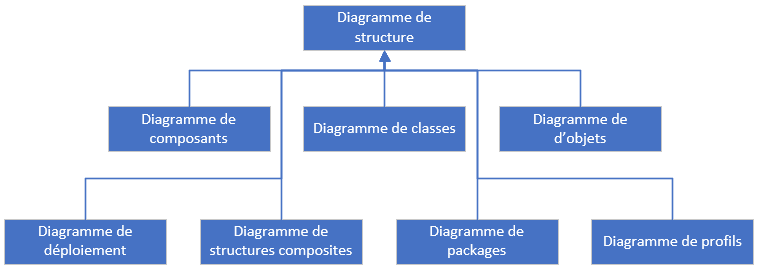
\includegraphics[width=12cm]{10_img/chap4/structure.PNG}
    \caption{Diagrammes de structure dans UML \cite{OMG_UML}}
    \label{fig.uml_struc}
\end{figure}

\begin{figure}[H]
    \centering
    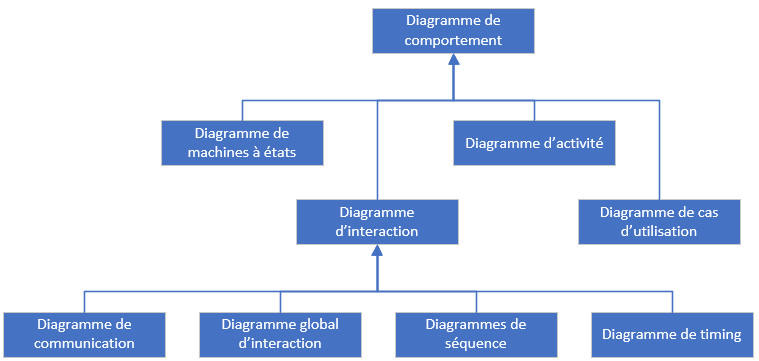
\includegraphics[width=12cm]{10_img/chap4/comportement.PNG}
    \caption{Diagrammes de comportement dans UML \cite{OMG_UML}}
    \label{fig.uml_comp}
\end{figure}

UML est un langage de modélisation connu et largement documenté dans le domaine de l'informatique.
Nous nous concentrerons plus particulièrement à définir les notions nécessaires à la compréhension des mécanismes et des éléments composant les profils UML.




\section{Le diagramme de profil UML}
Un profil UML est une forme de diagramme structurel décrit dans le standard UML.
Il permet d'étendre les mécanismes d'UML afin d'adapter les diagrammes et leur contenu à un domaine (ex : domaines d'activité spécifique) ou une plateforme particulière (ex : .NET, J2EE).

Les extensions qu'un profil appliquées au langage UML permettent d'ajouter des caractéristiques aux éléments standards d'UML.
Elles ne permettent pas de retirer les caractéristiques des éléments pour ne pas aller à l'encontre de la sémantique standard d'UML.
Le profil se compose  de stéréotypes de tagged values et de contraintes qui s'appliquent aux éléments des modèles UML tels que les classes, les attributs, les opérations et les activités.

\subsection{Exemple d'application}
Afin de mieux comprendre les éléments qui composent un diagramme de profil nous allons mettre en place un exemple d'application au fur et à mesure de ce chapitre en y intégrant les éléments un par un.
Prenons l'exemple d'un diagramme devant représenter un tableau de bord d'une machine composé de trois boutons : Marche, Action, Arrêt.
Ils ont chacun un état "actif" ou "inactif".
Ils ont chacun leur action propre sur la machine qu'ils contrôlent : Marche démarre la machine, Action actionne la machine, Arrêt stop le fonctionnement de la machine.

\begin{figure}[H]
    \centering
    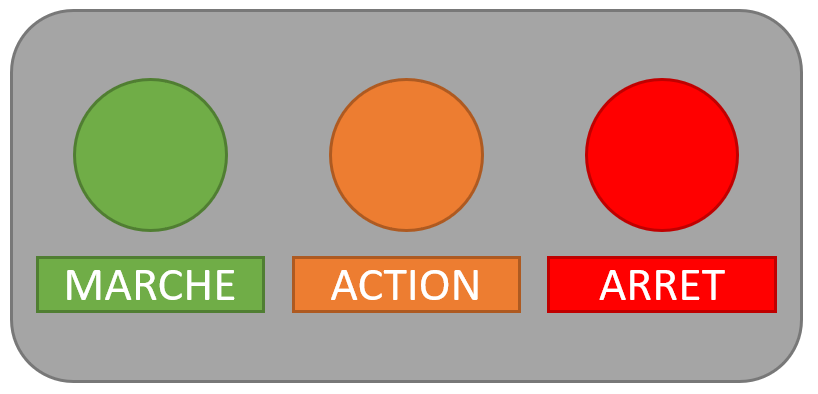
\includegraphics[width=8cm]{10_img/chap4/example.PNG}
    \caption{Tableau de bord de la machine}
    \label{fig.uml_ex}
\end{figure}

\newpage
\section{Les stéréotypes}
Les stéréotypes permettent d'appliquer des extensions aux métaclasse UML.
Il permettent d'ajouter des termes spécifiques de vocabulaire à un diagramme.
Un stéréotype s'applique à un objet UML permettant ainsi de le rendre spécifique à un domaine en y appliquant des propriétés spécifiques.

\subsection{Exemple d'application}
Dans notre exemple nous avons plusieurs éléments : un tableau de bord, des boutons, des actions que les boutons effectuent.
Un stéréotype, comme celui présent dans la figure \ref{fig.uml_but}, pourrait être créé afin de réunir les caractéristiques communes des boutons.


\begin{figure}[H]
    \begin{center}
    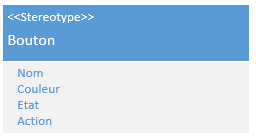
\includegraphics[width=5cm]{10_img/chap4/button.PNG}
    \caption{Stéréotype <<Bouton>> permettant de réunir les points communs des boutons}
    \label{fig.uml_but}
    \end{center}
\end{figure}


\newpage
\section{Les \emph{tagged values}}
Les \emph{tagged values} permettent d'ajouter des propriétés spécifiques au domaine d'application à un élément.
Cela permet d'ajouter de l'information spécifique aux éléments sous la forme clé/valeur.
Ces éléments se retrouvent appliqués au modèle entre crochets.

\subsection{Exemple d'application}
Dans notre exemple nous pouvons supposer que la machine est un modèle spécifique et donc que le diagramme ne s'applique qu'à ce modèle précis (ex : Modèle 1.2.3).
Nous trouverons donc dans notre diagramme UML la notation dans la figure \ref{fig.uml_mac}.

\begin{figure}[H]
    \begin{center}
    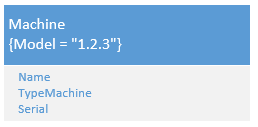
\includegraphics[width=5cm]{10_img/chap4/machine.PNG}
    \caption{\emph{Tagged value} permettant de spécifier le modèle de machine représenté}
    \label{fig.uml_mac}
    \end{center}
\end{figure}


\newpage
\section{Les contraintes}
Les contraintes sont des propriétés spécifiques aux profils UML qui permettent d'instaurer des conditions dans le modèle.
Ces conditions peuvent être appliquées à une ou plusieurs classes, à un ou plusieurs attributs, à un ou plusieurs relations entre classes.
Cette contrainte sera présente dans le modèle sous la forme d'une note comprenant la phrase exprimant la contrainte entre crochets.

\subsection{Exemple d'application}
Dans notre exemple nous pouvons supposer la contrainte suivante : l'action de la machine ne peut pas être effectuée si la machine est à l'arrêt.
Nous pourrons mettre en place dans notre diagramme UML la contrainte présente dans la figure \ref{fig.uml_con}.

\begin{figure}[H]
    \begin{center}
    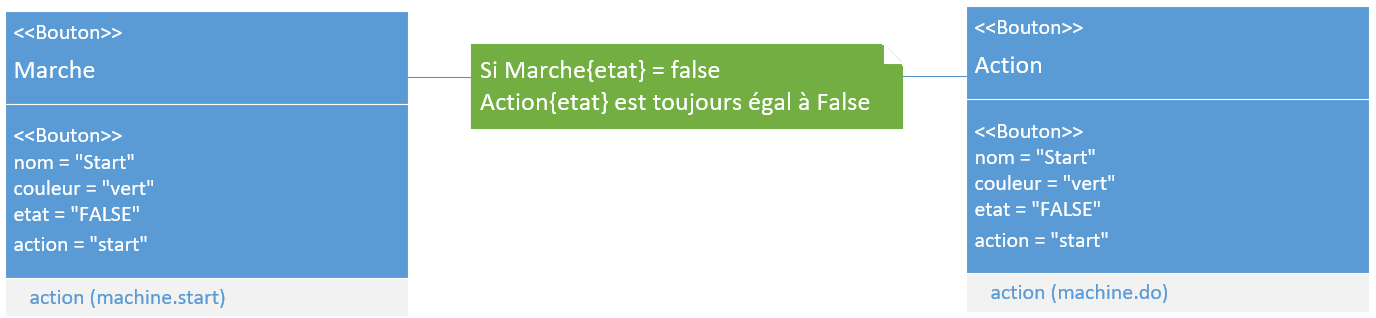
\includegraphics[width=12cm]{10_img/chap4/constraint.PNG}
    \caption{Contrainte permettant d'appliquer des conditions au modèle}
    \label{fig.uml_con}
    \end{center}
\end{figure}


\newpage
\section{Les images}
Lorsqu'un modèle devient important en taille il devient difficile de s'y retrouver.
Cependant l'application d'images aux modèles peut être une solution à mettre en place dans le cas d'un profil dans un domaine d'activité spécifique.
Une représentation graphique simple peut être attribuée à un type d'élément spécifique du modèle.

\subsection{Exemple d'application}
Dans notre environnement nous avons une machine composée de trois boutons.
Nous pouvons par exemple décider d'attribuer une image spécifique aux boutons afin de les différencier des autres éléments dans la figure \ref{fig.uml_img}.



\begin{figure}[H]
    \begin{center}
    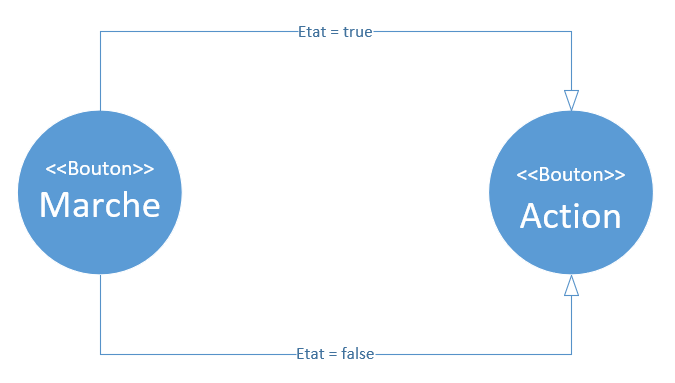
\includegraphics[width=12cm]{10_img/chap4/img.PNG}
    \caption{Image spécifique appliquée aux boutons dans le modèle}
    \label{fig.uml_img}
    \end{center}
\end{figure}


\newpage
\section{L'utilisation d'un profil UML pour la conception de jeux vidéos}


UML est un langage de modélisation permettant de représenter énormément de systèmes et permettant de les documenter de manière rigoureuse.

Permettre un \emph{mind mapping} à l'aide d'un outil tel qu'UML retirerait tous les désavantages d'un \emph{mind mapping} classique car :
\begin{itemize}
    \item UML est un langage formel et normalisé
    \item UML est manipulable ave de nombreux outils déjà approuvés
    \item UML est un support de communication performant
    \item UML est un langage qui permet le \emph{versionning} et la conservation de l'information de manière efficace
\end{itemize}


Cependant UML est un langage de modélisation tellement étendu qu'il permet de tout faire, cela rend le langage difficile à appréhender.
De plus UML est prévu à l'origine afin de représenter des systèmes logiciels, le vocabulaire utilisé est spécifique à la programmation informatique.


Dans les chapitres précédents nous avons établis une liste de points importants concernant la conception de jeux vidéos.
Nous pensons qu'un profil UML serait un outil adapté pour répondre aux besoins de modélisation d'un GDD.
La mise en place d'un profil UML permet de nombreux avantages :
\begin{itemize}
    \item Les outils sont nombreux et efficaces. Ils sont déjà présents sur le marché et répondent aux besoins de la modélisation UML
    \item Le scope des objets utilisables en UML est adaptable dans un profil ce qui permet de réduire la quantité de connaissances à acquérir pour se servir d'UML dans le cadre de la rédaction d'un GDD
    \item Les stéréotypes permettent d'intégrer le langage spécifique au \emph{game design}
    \item Les \emph{tagged values} permettent d'ajouter des propriétés spécifiques à chaque éléments
    \item Des contraintes peuvent être instaurées dans un profil afin d'éviter les erreurs
    \item Des images peuvent être appliquées aux éléments du modèle pour faciliter sa compréhension
\end{itemize}


Grâce à tous les ajustement permis par les profils, UML semble être un langage approprié pour permettre la représentation graphique d'un GDD.
C'est pourquoi l'outil proposé dans le chapitre \ref{game-genesis.sect} est un profil UML permettant l'organisation des éléments d'un GDD.